\chapter{Experimental Vehicle}

In order to verify the approach we discuss in this theses, we needed a car-like robot which we could use for real-world testing. We took inspiration from the F1/10 competition \cite{F1/10}, the MIT RACECAR\footnote{https://mit-racecar.github.io/}, AutoRally\footnote{https://autorally.github.io/}, and other similar projects and we built a robot based on a chassis from an 1:10 scale \gls{RC} car with an on-board computer and a set of sensors. In this chapter, we will describe the hardware components we used to build a custom experimental fast moving car.

\section{Chassis}

We used chassis, steering servo, \gls{DC} motor, \gls{ESC}, and a ratio transmitter and receiver from an off-the-shelf \gls*{RC} car. We removed the plastic cover and some unnecessary parts attached to the chassis and we attached a thin plywood board on top of the chassis. We later mounted all of the electronics to the plywood board. Even though the weight of the battery and of the electronics is not negligible, the suspension of the vehicle is stiff enough to carry the weight without any significant roll and pitch changes during acceleration and cornering.

\begin{figure}[!tbp]%
	\centering
	\begin{subfigure}[t]{0.45\textwidth}
		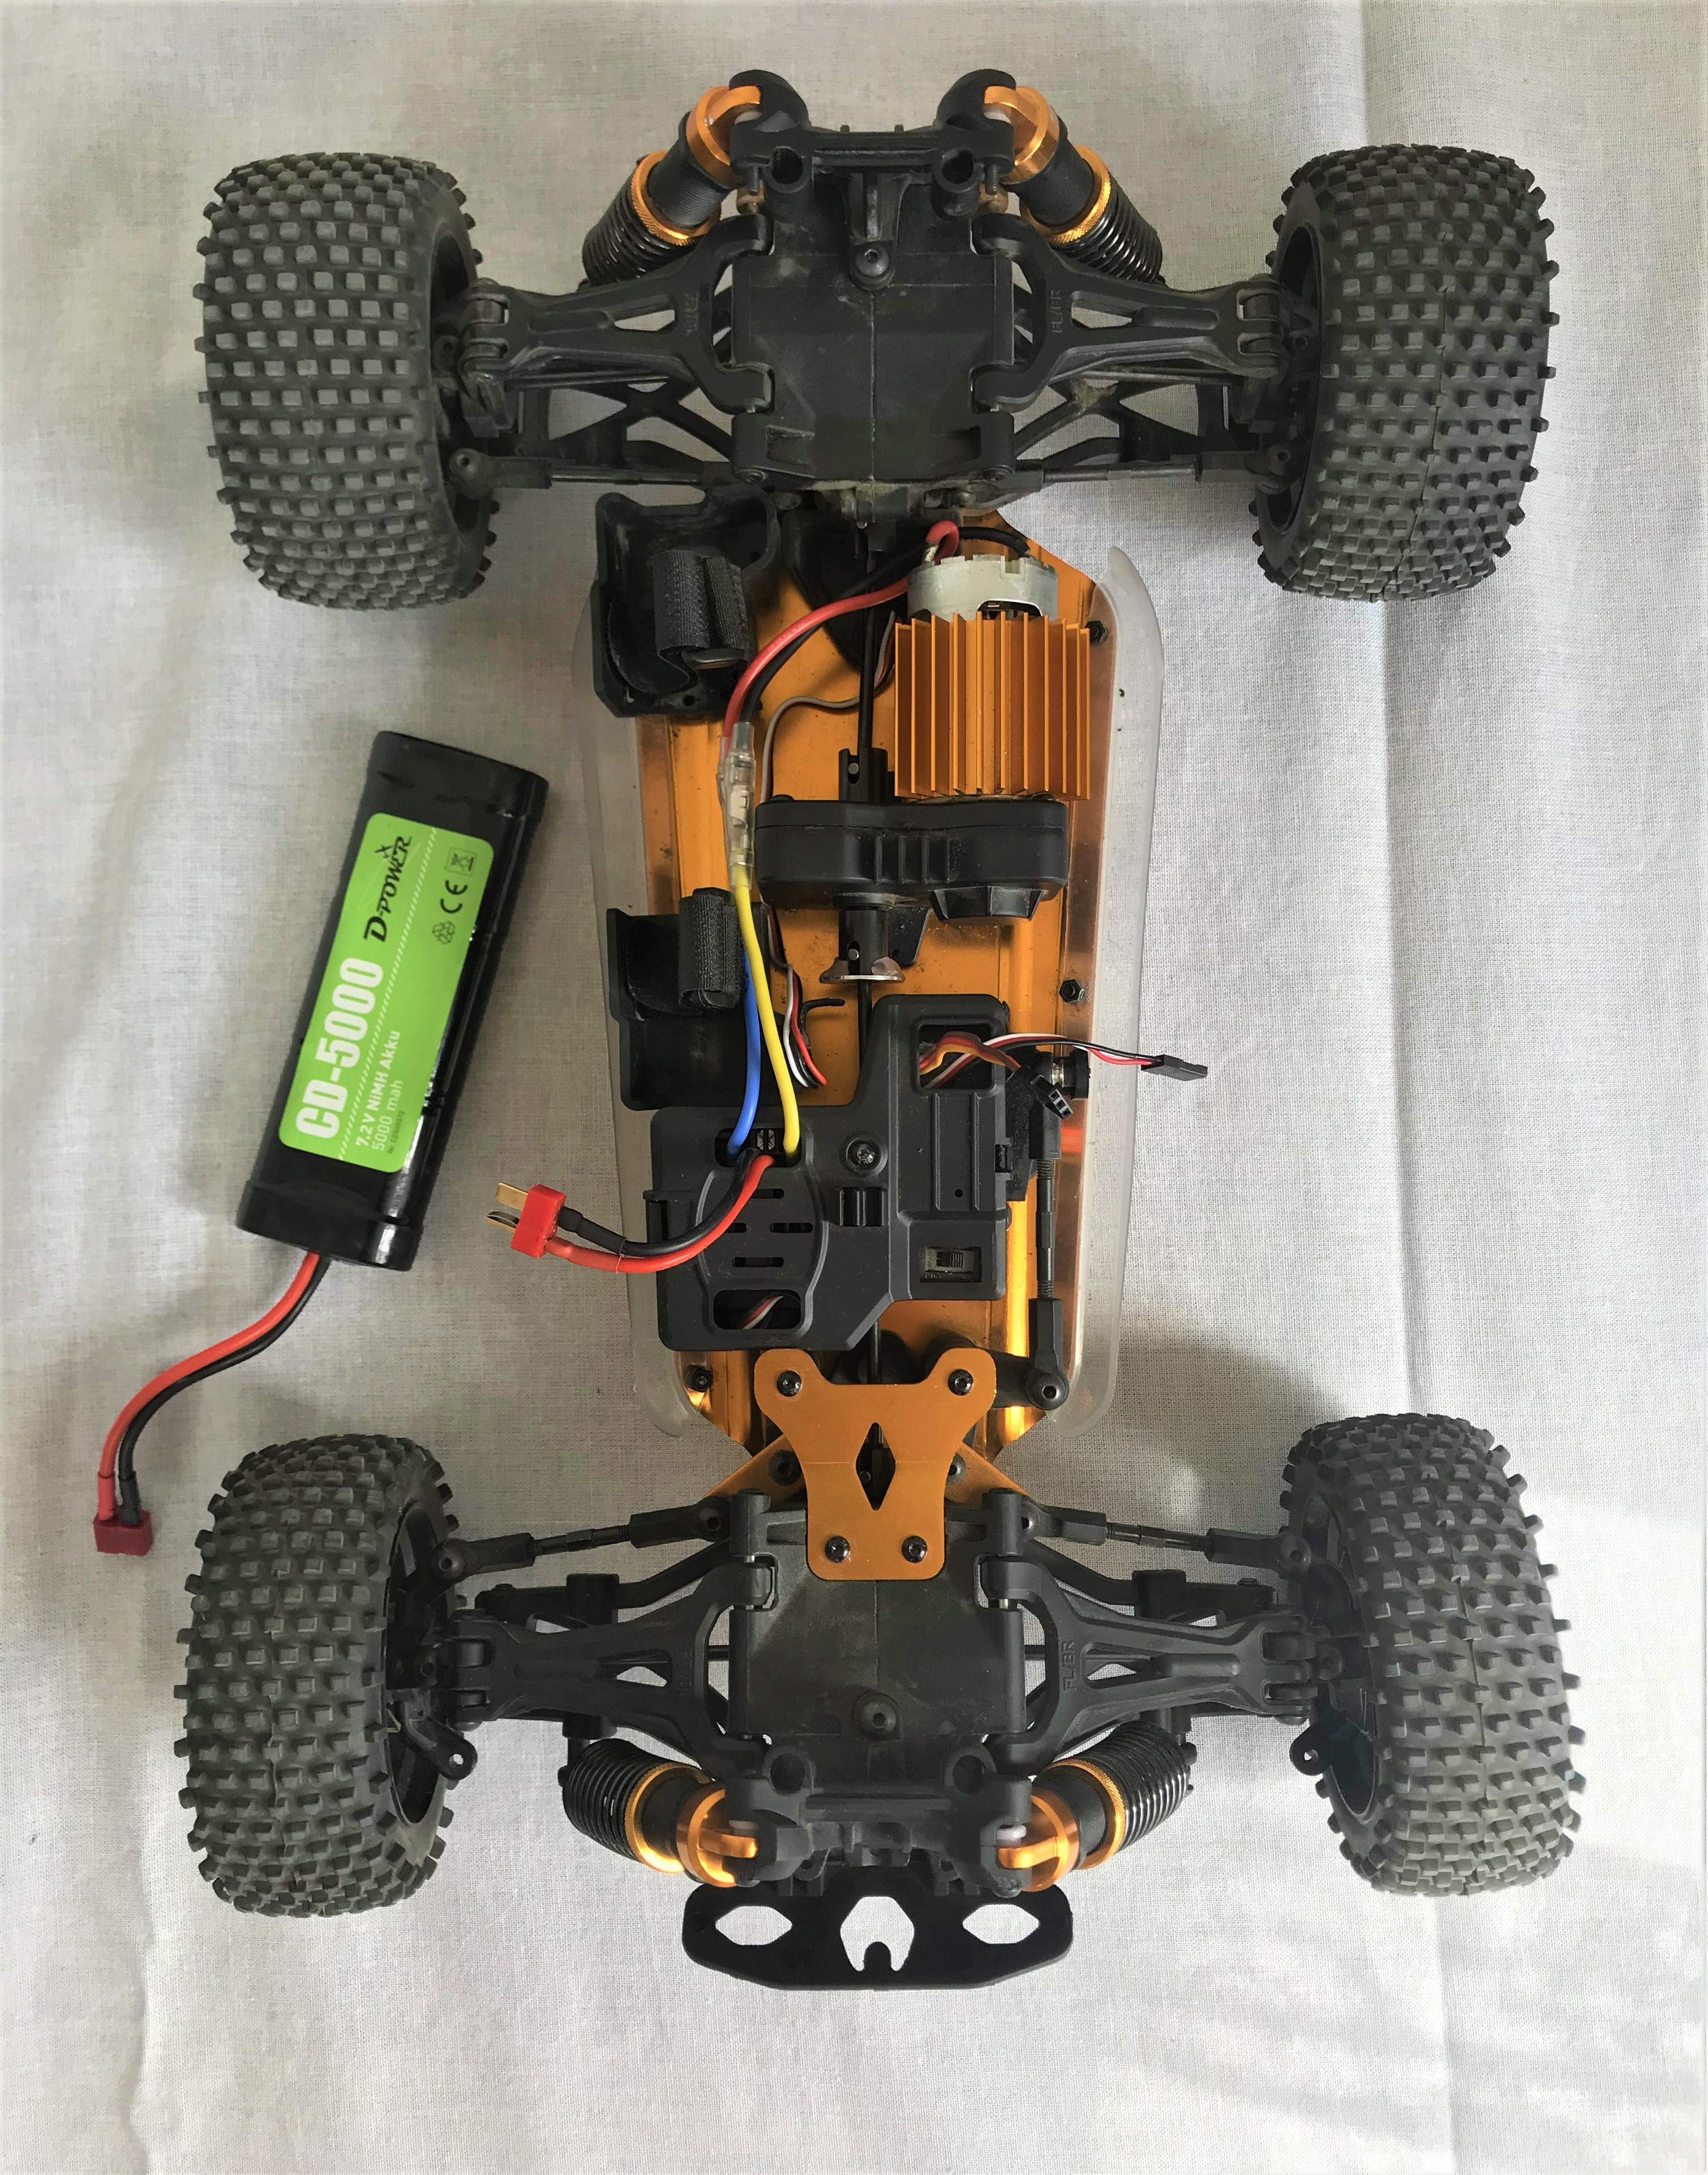
\includegraphics[width=\textwidth]{../img/car_top_no_electronics}
		\label{fig:chassis_no_electronics}
		\caption{A photo of the chassis of the vehicle without any additional electronics mounted to it.}
	\end{subfigure}
	\hfill
	\begin{subfigure}[t]{0.45\textwidth}
		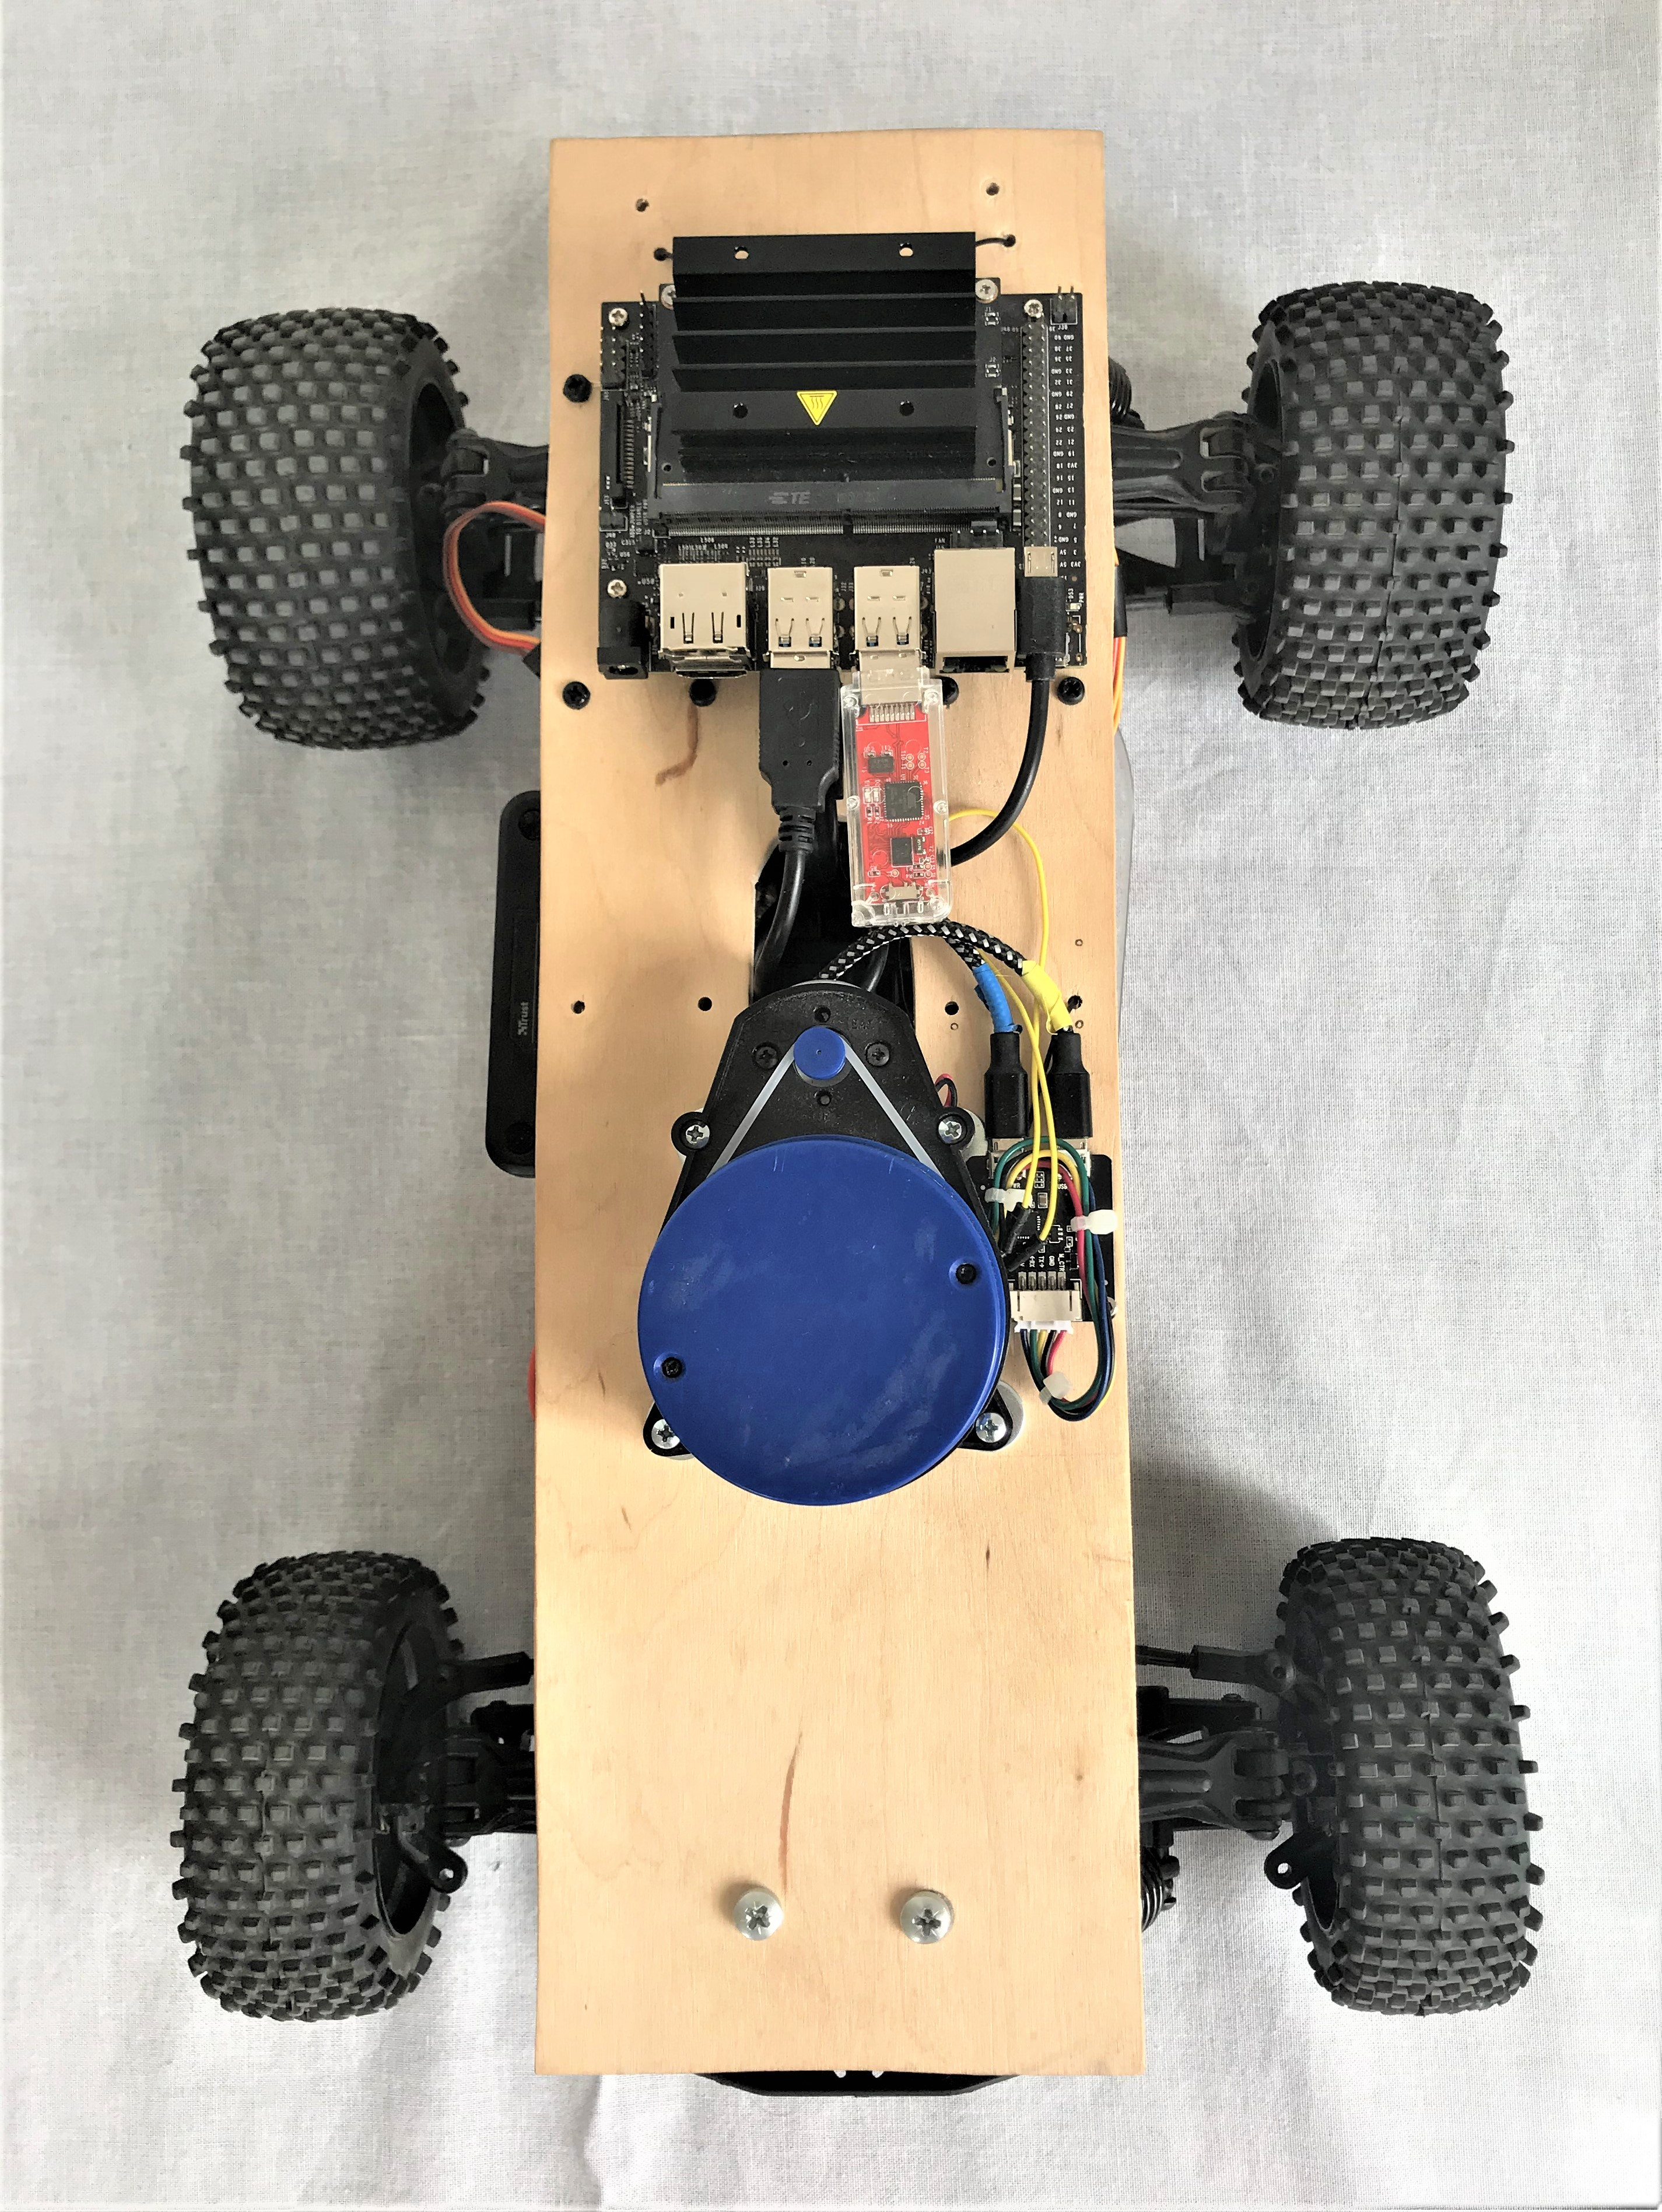
\includegraphics[width=\textwidth]{../img/car_top}
		\label{fig:chassis_with_electronics}
		\caption{A photo of the chassis with the plywood board with all of the electronics attached to it. Some of the components are not visible  because they are attached to the bottom side of the board.}
	\end{subfigure}

	\vspace{1cm}

	\begin{subfigure}[b]{0.7\textwidth}		
		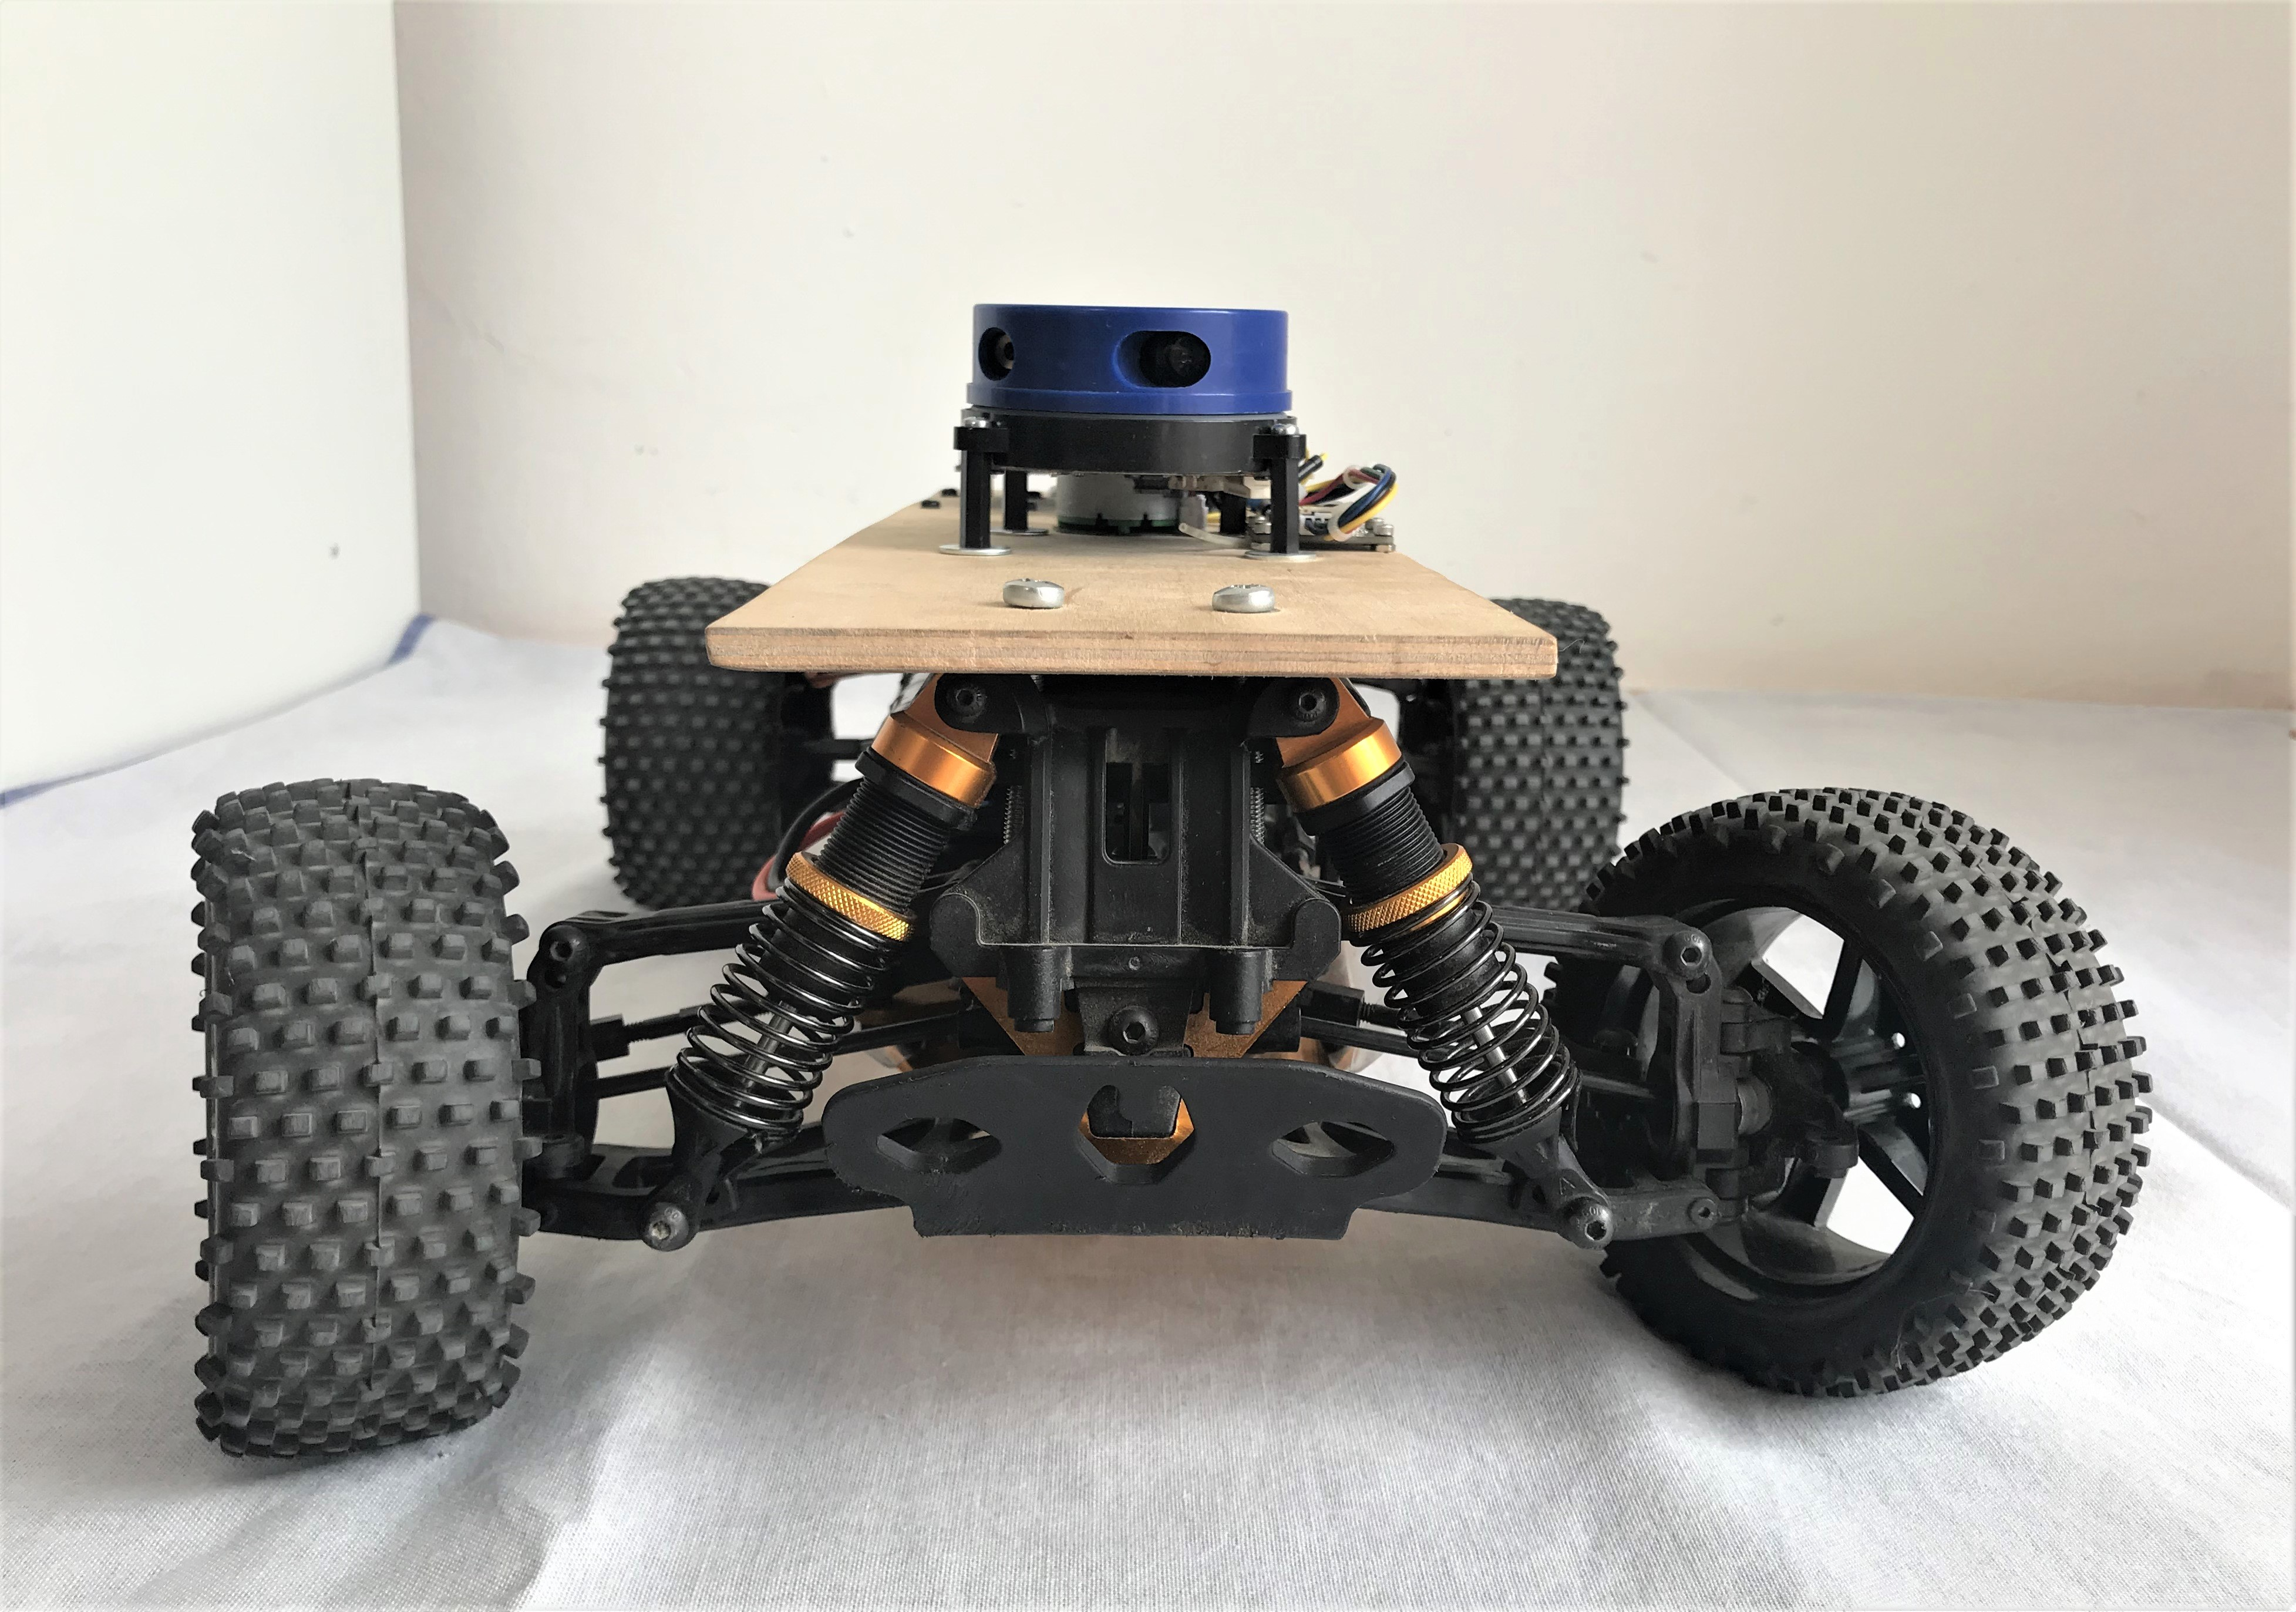
\includegraphics[width=\textwidth]{../img/car_front}
		\label{fig:chassis_front_view}
		\caption{Front view.}
	\end{subfigure}
	
	\label{fig:chassis}
	\caption{Photos of the experimental vehicle.}
\end{figure}

The chassis has the same geometry as a common passenger car with two fixed rear wheels and two front wheels with Ackermann steering geometry. All of the wheels are driven by the \gls*{DC} motor through a fixed gearbox. The wheels on both front and rear axes can move independently thanks to two differentials, one on each axis. The differentials are necessary for smooth travel during turns, when the outer wheel spins faster than the inner wheel. Photos of the vehicle are shown in Figure~\ref{fig:chassis}.

The steering servo and the \gls*{ESC}, which controls the speed of the \gls*{DC} motor, both have a 3-pin connector which was originally connected to a radio receiver. Two of the pins connect to a \gls*{DC} power supply and the third connects to a signal wire. The signal is originally created by an radio transmitter which generates a \gls{PWM} signal. The \gls*{PWM} signal consists of pattern resembling a square wave, where the voltage measured on the signal wire is high (\SI{5}{\volt}) for some period of time and then the voltage drops to low (\SI{0}{\volt}) for the rest of the period. The pulse of high voltage lasts between \SI{1}{\milli\second} and \SI{2}{\milli\second} and the period of the signal is \SI{20}{\milli\second} as it is shown in Figure~\ref{fig:pwm}. We can therefore connect these connectors to a computer which generates appropriate signals to steer the vehicle. The \SI{20}{\milli\second} period of one \gls*{PWM} cycle gives us an upper limit of \SI{50}{\hertz} at which we can change the commands for the vehicle.

\begin{figure}[]\centering
	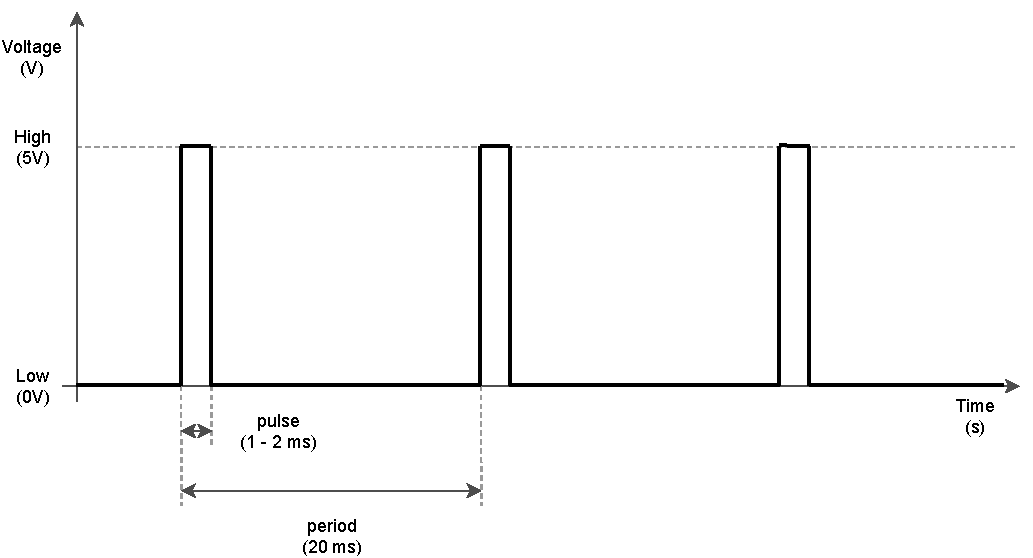
\includegraphics[width=125mm]{../img/pwm.pdf}
	\caption{The PWM signal for the steering servo and the ESC form a square wave with the period of \SI{20}{\milli\second} and pulse width between \SIlist{1;2}{\milli\second}.}
	\label{fig:pwm}
\end{figure}

\subsection{Servo Setting Time}

It takes non-trivial time for the steering servo to move from its previous position to a newly set position. The steering angle changes continuously as the servo adjusts and it affects the direction in which the vehicle travels in the meantime. In this experiment, we measure the setting time of the servo between different steering angles and based on the data, we will find a relationship between the distance between the servo position and the time it will take to set.

The position of the servo is set through a \gls{PWM} value between \SI{1200}{\micro\second} (rightmost position), \SI{1500}{\micro\second} (center position), and \SI{1800}{\micro\second} (leftmost position). In this procedure, the vehicle switches between a right position $r$ and a left position $l$ a hundred times while the vehicle is stationary and it is placed on a flat surface. The servo produces a noise during the whole setting period and is mostly quiet during the periods between adjustments.

We record the sound the servo makes through a microphone. The audio track is then edited using \textit{Audacity}\footnote{https://www.audacityteam.org/} to remove background noise and low frequency ``buzzing'' of the servo and to use the ``Sound Finder'' analysis tool to label periods of sound in the cleaned audio track (see Figure~\ref{fig:audacity}). The start and end times of the labeled intervals are then exported into a text file for further analysis.

We carried out this procedure for five pairs of \gls*{PWM} values: $(1800, 1200)$, $(1750, 1250)$, $(1700, 1300)$, $(1650, 1450)$, $(1600, 1400)$. Each of these pairs is symmetrical around the center position \SI{1500}{\micro\second} and the \textit{distance} between the two positions decreases from \SI{600}{\micro\second} to \SI{200}{\micro\second}. This might have biased the results and decrease the accuracy of our result.

\begin{figure}
	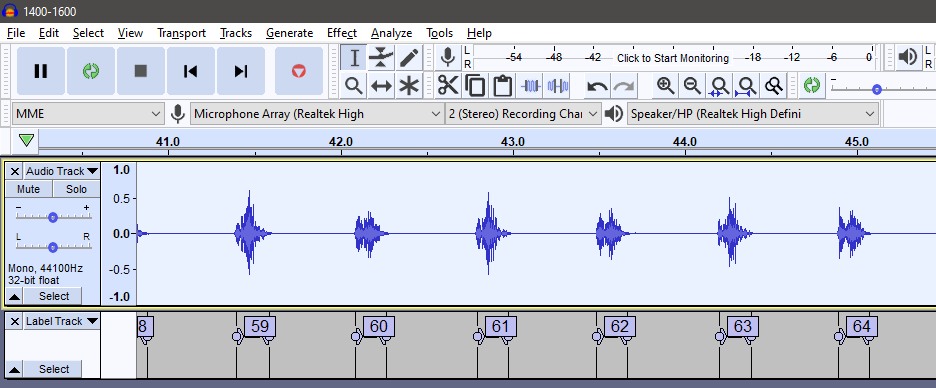
\includegraphics[width=\textwidth]{../img/servo_experiment_audacity}
	\protect\caption{The servo setting periods are clearly identifiable in an audio recording after background noise and low frequency sounds are removed. This figure shows the interface of the \textit{Audacity} tool used to analyze a recording of adjustments between the PWM signal of \SI{1400}{\micro\second} and \SI{1600}{\micro\second}.}
	\label{fig:audacity}
\end{figure}

We used the method of least squares to find a best fitting line in the form of $t=ad+b$, where $t$ is the setting time in seconds and $d$ is the distance between the \gls*{PWM} values. Based on the data we recorded, the relationship between the distance to the new servo position and the setting time is visualized in the Figure~\ref{fig:servo_linear_regression} and in the following equation:

\begin{equation}
\label{eq:servo_setting_time}
t(d)=0.000329\cdot d + 0.1174
\end{equation}

\begin{figure}
	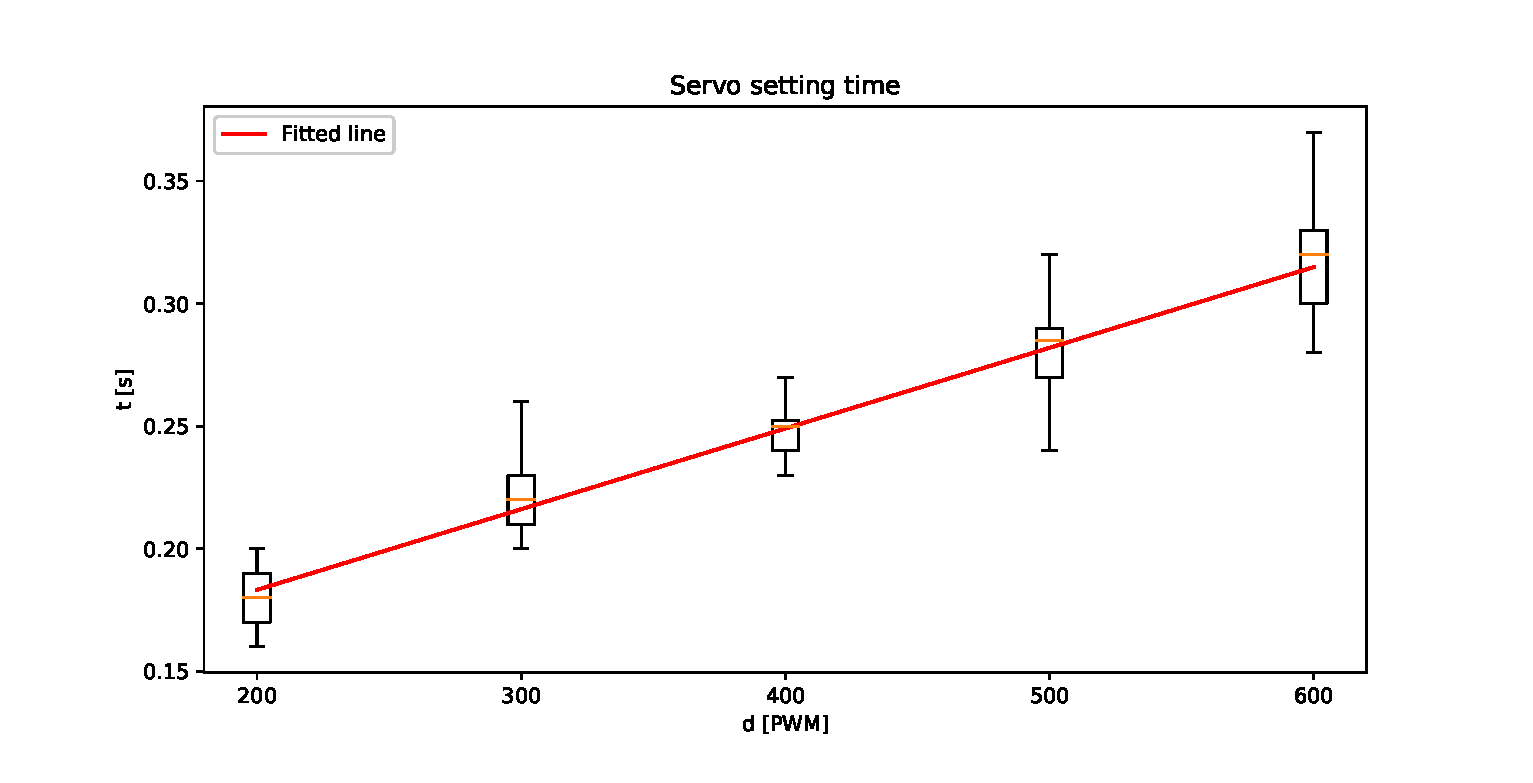
\includegraphics[width=\textwidth]{../img/servo_setting_time_linreg.eps}
	\caption{The setting time of the steering servo can be estimated with a linear function of the distance between the start and end PWM values.}
	\label{fig:servo_linear_regression}
\end{figure}

\subsection{Steering Angle to PWM Mapping}

The position of the steering servo is transferred to the front wheels through mechanical linkages. The inner wheel is steered more than the outer wheel, because the outer wheel will circumscribe a circle with a larger radius than the inner wheel. When the wheels are rolling perfectly against the surface at slow speed, the vehicle will keep going around a circle with a constant radius.

We measured the radius $R$ of the inner wheel as it circumscribes a circle, with the steering servo set to several constant \gls*{PWM} values. From this radius, we can calculate the steering angle $\delta$ of a virtual front wheel in the middle of the front axis from the geometry of the vehicle:

\begin{equation}
\delta=\arctan\left(\dfrac{L}{R+W/2}\right),
\end{equation}

where $L$ is the length of the wheelbase and $W$ is the width of the axles. The geometry is captured in Figure~\ref{fig:steering_angle_radius_geometry}. More information about Ackermann steering geometry can be found in \cite{Rajamani_lateral_dynamics}.\texttt{}

Using the least squares method, we identified a line which approximates the relationship between a steering angle and the \gls*{PWM} signal which corresponds to this angle:

\begin{equation}
	PWM(\delta)=12.701\cdot\delta + 1476.686,
\end{equation}

where $\delta\in\left[\ang{-21.16}, \ang{26.57}\right]$ is the steering angle expressed in degrees and $\ang{-21.16}$ is the maximum steering angle to the right and $\ang{26.57}$ is the maximum steering angle to the left. The relationship between the steering angle and the \gls*{PWM} value is shown in Figure~\ref{fig:steering_angle_to_pwm}.

\begin{figure}[h]
	\centering
	
	\begin{tikzpicture}[
	axis/.style={thin, densely dashed, gray},
	axle/.style={ultra thick, black},
	vec/.style={ultra thick, ->, >=latex}
	]

	\def\L{0.3} % wheelbase of the vehicle
	\def\W{0.3} % axle width
	\def\wW{0.05} % wheel width
	\def\wL{0.1} % wheel length
	\def\xoffset{3cm}
	\def\yoffset{0.8cm}
	\def\R{0.95}
	\def\stateDelta{17.52556837}
	
	\begin{scope}[scale=5]
	
	\coordinate (O) at (0, 0);
	\coordinate (front) at (\R, \L);
	\coordinate (rearRight) at (\R + \W/2, 0);
	\coordinate (frontRight) at (\R + \W/2, \L);

	% the circle	
	\draw[gray, dashed] (O) circle (\R);
	\draw[gray] (O) circle (\R - \W/2);
	
	% visualize delta
	\draw[thin] (front) -- ++(0, \L);
	\draw[thin, rotate around={\stateDelta:(front)}] (front) -- ++(0, \L);
	\draw (front)++(0, 0.2) arc (90:90+\stateDelta:0.2) node[above, xshift=1.6mm] {$\delta$};

	% visualiza the geometry
	\draw[thin, ->, >=latex] (O) -- node[below] {$R$} (\R - \W / 2, 0);
	\draw[thin] (O) -- (front);
	\draw (O)++(0.2, 0) arc (0:\stateDelta:0.2) node[right, yshift=-1.3mm, xshift=1mm] {$\delta$};

	% longitudinal axle
	\draw[axle] (\R, 0) -- ++(0, \L);
	
	% visualize the wheelbase length
	\draw[axis] (rearRight) -- ++(0.25, 0);
	\draw[axis] (frontRight) -- ++(0.25, 0);		
	\draw[<->, >=latex] ($ (rearRight) + (0.2, 0) $) -- node[right] {$L$} ($ (frontRight) + (0.2, 0) $);
	
	% visualize the width length
	\draw[axis] (\R - \W/2, 0) -- ++(0, -0.25);
	\draw[axis] (\R + \W/2, 0) -- ++(0, -0.25);		
	\draw[<->, >=latex] (\R - \W/2, -0.2) -- node[below] {$W$} (\R + \W/2, -0.2);
	
	% rear axle
	\draw[axle] (\R - \W/2, 0) -- ++(\W, 0);
	\filldraw[] (\R - \W/2, -\wL/2) rectangle ++(\wW, \wL);
	\filldraw[] (\R + \W/2 - \wW, -\wL/2) rectangle ++(\wW, \wL);
	
	% front axle
	\def\deltaL{\stateDelta + 3}
	\def\deltaR{\stateDelta - 2}
	\draw[axle] (\R - \W/2, \L) -- ++(\W, 0);
	\filldraw[rotate around={\deltaL:(\R - \W/2 + \wW/2, \L)}] (\R - \W/2, \L - \wL/2) rectangle ++(\wW, \wL); % front left wheel/tire
	\filldraw[rotate around={\deltaR:(\R + \W/2 - \wW/2, \L)}] (\R + \W/2 - \wW, \L - \wL/2) rectangle ++(\wW, \wL); % front right wheel/tire

	\end{scope}
	\end{tikzpicture}
	
	\caption{For a fixed steering angle $\delta$ of the virtual front center wheel, the vehicle will move along a circle of radius $R$, unless the wheels start skidding. The proportions of the vehicle in the picture are the same as on the experimental vehicle, where $W=L=\SI{0.3}{\meter}$.}
	\label{fig:steering_angle_radius_geometry}
\end{figure}

\begin{figure}
	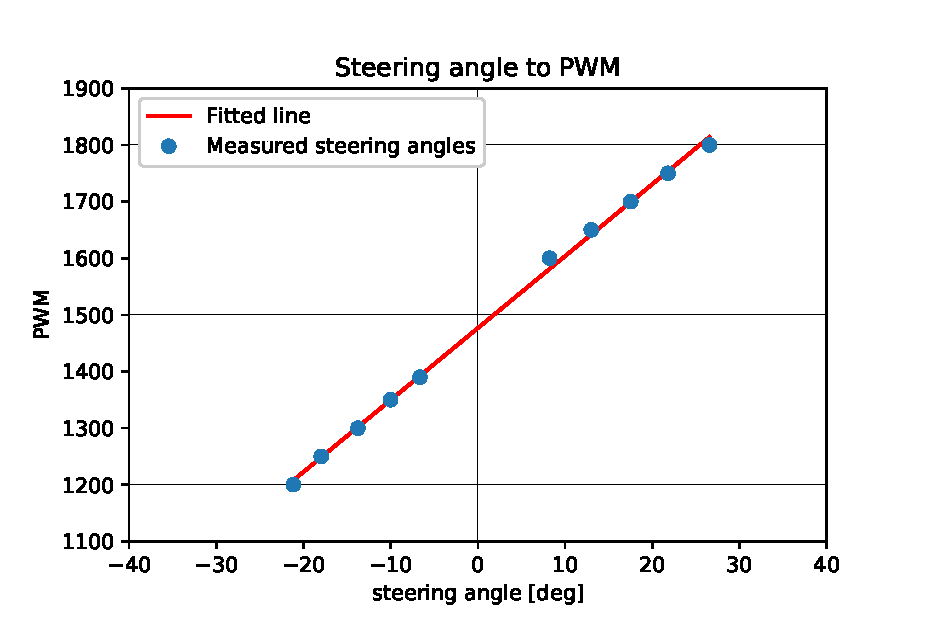
\includegraphics[width=\textwidth]{../img/steering_angle_to_pwm}
	\caption{The measurement shows the imperfections in the hardware construction. The vehicle is able to go around circles with smaller radii when it is turning left (positive steering angles) than when it is turning right (negative steering angles).}
	\label{fig:steering_angle_to_pwm}
\end{figure}

\subsection{DC Motor Model}

We need to be able to model the angular velocity of the motor shaft. The motor is directly connected to the wheels. Therefore, if we can predict the velocity at which the motor shaft rotates, we can predict how fast the wheels will turn. This, of course, does not give us all the information to determine the longitudinal velocity of the vehicle, because the wheels might skid when the friction forces between the tires and the road surface are exceeded.

Our goal is to create a model of the engine RPM as a function of the previous \gls{RPM} and the control inputs. We measured the RPM of the motor shaft using a Hall effect encoder while we were manually controlling the vehicle on dry asphalt at a temperature of around \SI{15}{\degreeCelsius}. We also recorded the throttle and steering angle inputs from the remote control. We use the collected data to identify the parameters of our model and to validate the accuracy of the model.

The torque of the motor depends directly on the speed at which its axle rotates. For a DC motor, the relationship can be approximated with a linear function which depends on two parameters: the maximum angular velocity $\omega_{max}$ and stall torque $T_{stall}$ as it is shown in Figure~\ref{fig:torque_rpm_curve}. The maximum angular velocity is measured with full throttle when there is no load on the motor and the stall torque is reached when the vehicle starts moving from standstill.

The throttle control input $\tau_t$ limits the amount of torque transferred to the wheels. The torque is counteracted by the load on the motor, e.g., friction or air resistance. While driving the experimental car manually, we learned that the steering angle $\delta_t$ of the front wheels is one of the most significant factors limiting the speed of the motor. When the car is at its maximum speed and the throttle is released, the car will travel a significant distance before it comes to a full stop. When the steering angle is large, the car stops almost immediately. The vehicle reaches a lower speed when it travels around a circle compared to going straight when full throttle is applied. The rate of change of angular velocity of a rigid body is equal to the total torque applied to the body divided by its moment of inertia.

We model the rate of change of the angular velocity of the motor with the following set of parametric equations, which are inspired by the mechanics of the motor:

\begin{equation}
\begin{aligned}
\label{eq:motor_model}
T(\omega)&=\left(1 - \dfrac{\omega}{\omega_{max}}\right)x_1 \\
T_{drive}(\tau_t, \omega)&=T(\omega)\cdot \tau_t \\
T_{load}(\delta_t, \omega)&=\omega^{x_2} \left(x_3 + x_4|\delta_t|\right)^{x_5} \\
\dot{\omega}(\omega, \tau_t, \delta_t)&=\dfrac{T_{drive}(\tau_t, \omega)-T_{load}(\delta_t, \omega)}{x_6}.
\end{aligned}
\end{equation}

The parameters $x_i\in\mathbb{R}$ are obtained using a numerical optimization algorithm which minimizes mean squared error between the predicted RPM and RPM measured using the experimental vehicle. The parameter $x_1$ replaces $T_{stall}$ and $x_6$ replaces the moment of inertia of the power train. Nevertheless, the values assigned to these parameters by the optimization algorithm must not be interpreted as the values of these two properties.

By integrating the $\dot{\omega}$ numerically over a time period $\Delta t$, we will obtain the change in the RPM of the vehicle. The performance of our model with fitted parameters is shown in Figure~\ref{fig:motor_rpm_model} for a time period of almost two minutes. The \gls*{RPM} shown in this figure is relative to the maximum \gls*{RPM} of the motor, which we identified to be \SI{15500}{RPM}.

We also tried training a neural network with three input neurons and one output neuron to predict $\dot{\omega}$ or $\omega$ directly. We experimented with supervised learning and with reinforcement learning using neuro-evolution (NEAT) but we were not able to obtain a neural network with better estimates of $\omega$ than the predictions from the model described in (\ref{eq:motor_model}).

\begin{figure}
	\centering
	
	\begin{tikzpicture}
	
	% the axes
	\draw[thick, ->] (-1,0)--(8,0) node[right]{$RPM$};
	\draw[thick, ->] (0,-1)--(0,6) node[above]{$torque$};
	
	\draw[ultra thick] (0, 4.5) node[left]{$T_{stall}$}--(7, 0)node[below]{$\omega_{max}$};
	
	\end{tikzpicture}
	
	\caption{Linear approximation of a DC motor torque curve. This linear model has two parameters: the maximum RPM without any load $\omega_{max}$ and stall torque $T_{stall}$.}
	\label{fig:torque_rpm_curve}
\end{figure}

\begin{figure}
	\centering
	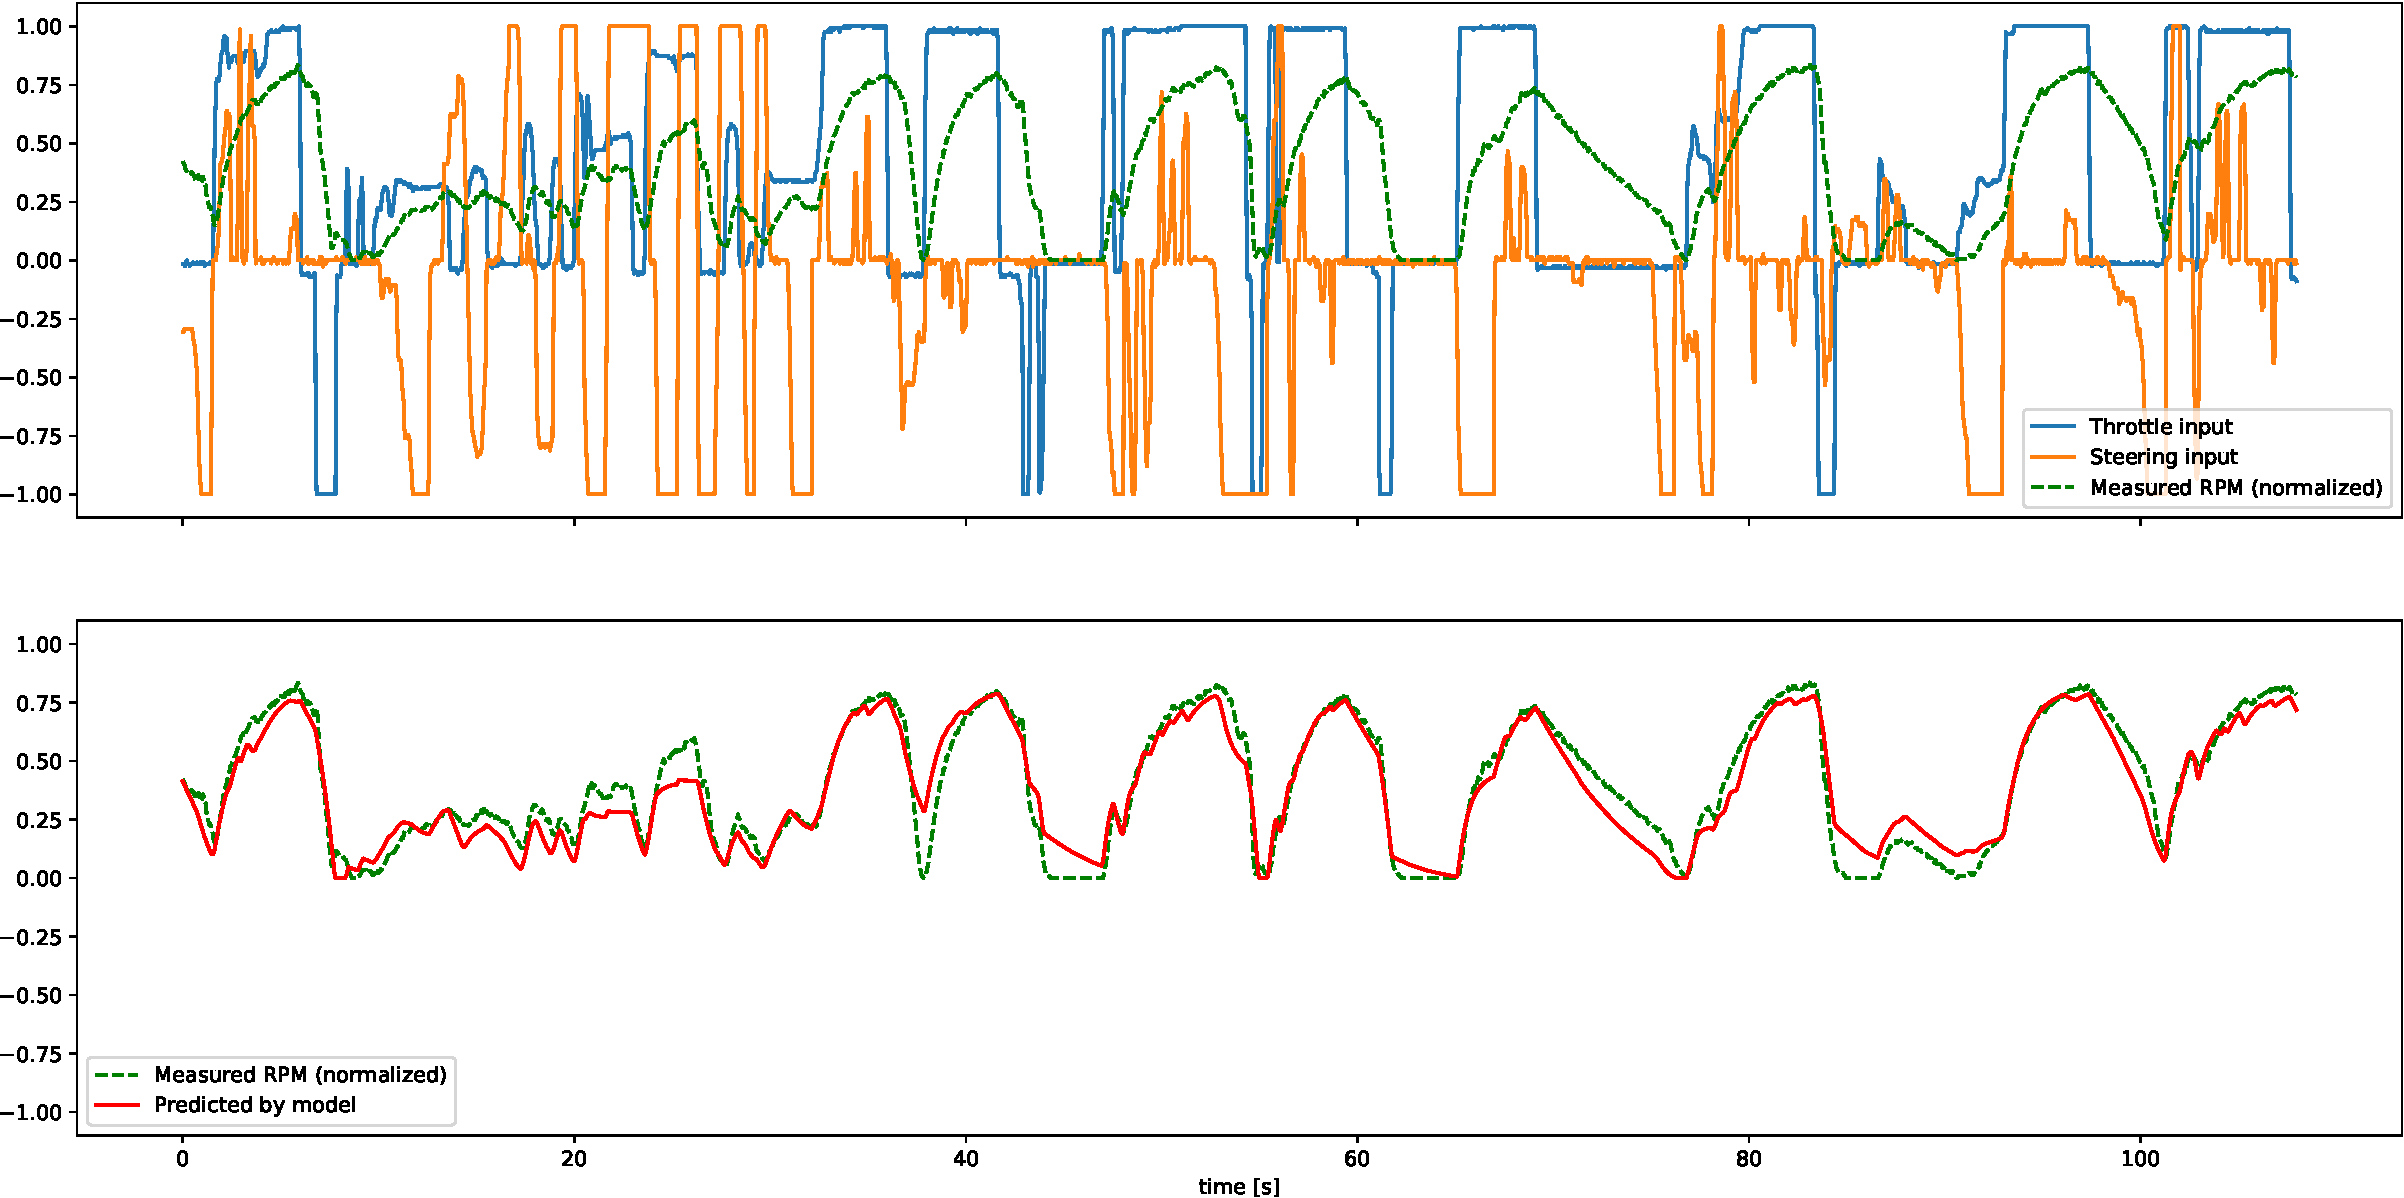
\includegraphics[width=\textwidth]{../img/fit_8000}
	\caption{The first chart shows the throttle and steering inputs as well as the measured RPM (normalized). The second chart compares the measured and predicted RPMs for the same time period using the fitted parameters of our model.}
	\label{fig:motor_rpm_model}
\end{figure}

\section{Sensors}

The vehicle uses on-board sensors to track its location on the racing track. We use a combination of three sensors: a \gls{LIDAR}, an \gls{IMU}, and a motor encoder. We tried several different sensors from different manufacturers, including \verb|Razor 9DoF IMU| and \verb|Scanse Sweep 2D LIDAR|, but these devices did not yield good results. 

\paragraph{Hall Effect Encoder} consists of an 8-pole magnetic disc which we attach to the drive shaft of the vehicle, and a Hall effect sensor. The sensor sends a pulse every time it detects a change from a north pole to a south pole or vice-versa. This way we can detect that the motor has made one eigth of a revolution. By counting the number of revolutions and by assuming that the wheels of the vehicle roll perfectly against the road surface, we can estimate the distance that the vehicle traveled. By combining this information with the current steering angle of the front wheels, we can estimate the movement of the vehicle and use it as a source of odometry. We used a ``Wheel Encoder Kit from DAGU'' from SparkFun\footnote{https://www.sparkfun.com/products/12629}.

\paragraph{Bosch BNO055 USB Stick} is an \gls{IMU} which contains a triaxial accelerometer, a triaxial gyroscope, a triaxial magnetometer and a thermometer\footnote{https://www.bosch-sensortec.com/bst/products/all\_products/bno055} . We use the measurements of the gyroscope and the accelerometer to determine the acceleration of the vehicle to improve our odometry from the motor encoder, which cannot detect wheel skidding.

\paragraph{YDLIDAR X4} is a low-cost \ang{360} \gls{LIDAR} laser scanner. We use it to determine the distance to the surrounding obstacles. This sensor has a range of up to \SI{10}{\meter} and it takes \num{5000} samples every second while spinning at the frequency of almost \SI{12}{\hertz}. This sensor is connected to a computer via a micro-USB port and it is connected to a \SI{5}{\volt} power supply through a second micro-USB port.

\section{On-board Computer}

The brains of our autonomous vehicle is the NVIDIA Jetson Nano\footnote{https://developer.nvidia.com/embedded/jetson-nano-developer-kit} . This board contains a quad-core ARM A57 with the clock frequency of \SI{1.43}{\giga\hertz}, \SI{4}{\giga B} of LPDDR4 RAM and a 128-core Maxwell GPU. This computer is powered through a Micro-USB port with \SI{5}{\volt}/\SI{2}{\ampere}\footnote{The board can operate with a lower power consumption of \SI{5}{\watt} in a mode in which two of the CPU cores are turned off.}. The Jetson has 4 USB ports which are used to connect the \gls*{LIDAR}, the \gls*{IMU}, and two Arduino boards. The board does not include a Wi-Fi antena and therefore we added an Intel Dual Band Wireless-Ac 8265 W/Bt card to the M.2 slot of the board in order to receive telemetry while the vehicle is driving along a circuit.

\subsection{Microcontrollers}

We use two Arduino Nano boards\footnote{https://www.arduino.cc/en/Guide/ArduinoNano} as an interface between the actuators, the radio receiver, and the motor encoder, and the Jetson Nano board.

\paragraph{Hall Effect Encoder} is connected to an interrupt pin of one Arduino and this Arduino counts the number of revolutions of the motor. This board also provides power to the Hall sensor.

\paragraph{ESC and Servo} are connected to \gls{PWM} output pins of the other Arduino board and the radio receiver is connected to two interrupt pins. This board contains logic which converts high-level commands for the actuators into corresponding \gls*{PWM} signals. It also contains a safety mechanism which disables autonomous mode of the vehicle and allows the supervisor to take over control of the vehicle when he or she uses the remote controller.

\section{Power Supply}

The \gls*{DC} motor and the servo are powered by \SI{7.2}{\volt} \SI{5000}{\milli\ampere\hour} NiMH battery which was included with the \gls*{RC} car. The rest of the electronics of the vehicle is powered by a regular \SI{20000}{\milli\ampere\hour} power bank which has two output USB ports. One of these ports can supply \SI{2}{\ampere} and the Jetson Nano board is connected to it, the other port can supply \SI{1}{\ampere} and it powers the \gls*{LIDAR}.

This setup ensures that the power in the batteries supplying the motors of the vehicle discharge much sooner than the power bank which supplies the computer and sensors if we start with fully charged batteries. It should never occur that the computer shuts down while the car is being driven autonomously and it will not continue moving uncontrollably. We also do not need to build a custom power delivery board.
